\documentclass[10pt,a4paper]{ctexart}
\usepackage[margin=2cm]{geometry}
\usepackage{graphicx}
\usepackage{diagbox}
\usepackage{float}      % 支持 [H] 浮动体选项
\usepackage{hyperref}
\usepackage{amsmath}    % 提供方程环境
\usepackage{physics}    % 简化向量、微分算子语法
\usepackage{siunitx}    % 提供 \ang 和 \SI 命令
\newcommand{\myspace}[1]{\par\vspace{#1\baselineskip}} %自定义空一行
\usepackage{fancyhdr}
\usepackage{booktabs}
\usepackage{caption}
\pagestyle{fancy}
\fancyhf{}  % 清除所有页眉页脚
\fancyfoot[C]{\thepage}  % 在页脚中央设置页码
\renewcommand{\headrulewidth}{0pt}  % 去掉页眉横线
\renewcommand{\footrulewidth}{0pt}  % 去掉页脚横线

\usepackage{hyperref}
\hypersetup{
    colorlinks=true,
    linkcolor=blue,
    filecolor=magenta,      
    urlcolor=cyan,
    pdftitle={Overleaf Example},
    pdfpagemode=FullScreen,
    }

\usepackage{titlesec}

% 重新定义section格式
\titleformat{\section}
  {\normalfont\Large\bfseries}
  {\chinese{section}、}
  {0pt}
  {}

% 给出常用字号的自定义指令
\newcommand{\chuhao}{\fontsize{42pt}{48pt}\selectfont}
\newcommand{\xiaochu}{\fontsize{36pt}{42pt}\selectfont}
\newcommand{\xiaoer}{\fontsize{18pt}{21.6pt}\selectfont}
\newcommand{\sanhao}{\fontsize{16pt}{20pt}\selectfont}
\newcommand{\xiaosan}{\fontsize{15pt}{18pt}\selectfont}
\newcommand{\sihao}{\fontsize{14pt}{18pt}\selectfont}
\newcommand{\xiaosi}{\fontsize{12pt}{16pt}\selectfont}
\newcommand{\wuhao}{\fontsize{10.5pt}{12.6pt}\selectfont}

% 定义中文数字转换
\titleformat{\section}
  {\normalfont\Large\bfseries}
  {\zhnum{section}、}  % 使用\zhnum而不是\chinese
  {0pt}
  {}

% 标题设置
\title{\xiaochu\textbf{物理实验报告}}
\author{}
\date{}

\begin{document}

\vspace*{36pt} % 顶部空白

% 居中填写区域
\begin{center}
    
\includegraphics[width = 9cm]{figure/head.png}
    
    \xiaochu\textbf{物理实验报告}
    % 预留空白区域
    \vspace{13pt}
    \vspace{13pt}
    \vspace{13pt}
    \vspace{13pt}
    
    \sanhao\textbf{实验名称：\underline{\makebox[10cm]{ 光的偏振研究}}} \\[10pt]
    \sanhao\textbf{实验桌号：\underline{\makebox[10cm]{ 16}}} \\[10pt]
    \sanhao\textbf{指导教师：\underline{\makebox[10cm]{ 姜柏旭 }}} \\[30pt]
    
    % 预留空白区域
    \myspace{6}
    
   \sihao\textbf{班级：\underline{\makebox[6cm]{}}} \\[10pt]
    \sihao\textbf{姓名：\underline{\makebox[6cm]{}}} \\[10pt]
    \sihao\textbf{学号：\underline{\makebox[6cm]{}}} \\[30pt]
    
   \sihao\textbf{实验日期: 
   \underline{\makebox[0.8cm]{2025}}  年 
   \underline{\makebox[0.4cm]{12}}月
   \underline{\makebox[0.4cm]{3}}日  
   星期\underline{\makebox[0.6cm]{三}}上午}
    
    \vspace{18pt}
    \sihao 浙江大学物理实验教学中心
    
\end{center}

\newpage

\section{预习报告}

    \subsection{实验综述}
    
    \xiaosi （自述实验现象、实验原理和实验方法，不超过300字，5分）
 
    光虽然本质是电磁波，有电场和磁场两个分矢量，但是引起视觉效应的主要是电场矢量的振动方向。
    自然光的电场矢量在垂直于传播方向的各个方向上均匀振动，称为非偏振光；
    如果电场矢量只在某一特定方向上振动，则称为偏振光。
    偏振光可以通过反射、折射、散射等方法产生，也可以通过一些光学器件如偏振片、双折射晶体等获得。

    反射产生的偏振光现象称为布儒尔偏振现象，当光线以某一特定角度（布儒斯特角）入射到介质界面时，反射光完全偏振并与折射光垂直。
    本实验通过如下图的实验装置观察布儒尔偏振现象，测量布儒斯特角并得到介质的折射率；

\begin{figure}[H]
    \centering
    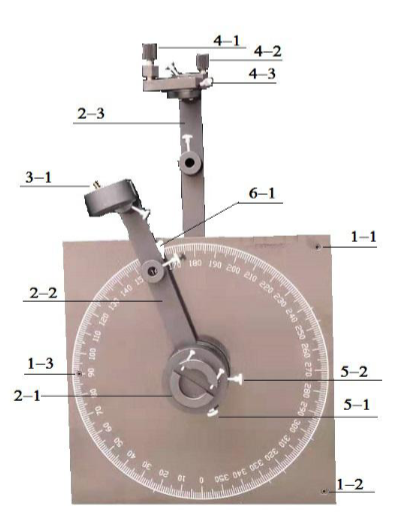
\includegraphics[width=0.6\textwidth]{figure/ex.png}
    \caption{布儒尔偏振现象实验装置示意图}
\end{figure}
    之后通过使光线以布儒斯特角入射，调整偏振片的转动角度，使光强出现极大和极小来测量偏振片的偏振化方向角度。
\myspace{2}
    
实验通过改变偏振片角度和测量光强的关系，验证马吕斯定律，即通过偏振片后的光强与入射光强和偏振片夹角的平方成正比关系并研究硅光电池的光电流和光强的关系。
    \myspace{2}
    
    
    \subsection{实验重点}
    
    \xiaosi（简述本实验的学习重点，不超过100字，3分）
    
 (1)利用布儒斯特角测量黑色平板折射率

    (2)测量偏振片的偏振化方向角度

    (3)验证马吕斯定律,研究硅光电池的光电流和光强的关系
    \myspace{2}
    
    \subsection{实验难点}
    
    \xiaosi（简述本实验的实现难点，不超过100字，2分）

(1)调节光路，使入射光线以布儒斯特角入射到介质界面；

    (2)准确测量偏振片的偏振化方向角度；

    (3)验证马吕斯定律时，准确测量不同偏振片角度下的光强值。

    (4)调整器件等高共轴
    
    (5)测量折射率时准确确定光强最小的角度
\myspace{2}
\section{原始数据}

    \xiaosi （将有老师签名的“自备数据记录草稿纸”的扫描或手机拍摄图粘贴在下方，20分）
   
\begin{figure}[H]
    \centering
    
\includegraphics[width=0.8\textwidth]{figure/raw_data.jpg}
    \caption{实验原始数据记录}
\end{figure}
\section{结果与分析}

    \subsection{数据处理与结果}
    \xiaosi （列出数据表格、选择数据处理方法、给定测量或计算结果，30分）

\subsubsection{测量黑色平板折射率}
\begin{table}[H]
\centering
\caption{测量黑色平板折射率}
\label{tab:n}
\begin{tabular}{|l|l|l|l|}
\hline
组数 & \begin{tabular}[c]{@{}l@{}}左侧角坐标\\ $\theta_1$\end{tabular} & \begin{tabular}[c]{@{}l@{}}右侧角坐标\\ $\theta_2$\end{tabular} & 布儒斯特角 \\ \hline
1 & \ang{74.1} & \ang{290.1} & \ang{54.0} \\ \hline
2 & \ang{75.0} & \ang{288.5} & \ang{53.4} \\ \hline
3 & \ang{75.1} & \ang{291.2} & \ang{54.0} \\ \hline
4 & \ang{76.0} & \ang{292.0} & \ang{54.0} \\ \hline
5 & \ang{75.5} & \ang{291.9} & \ang{54.1} \\ \hline
6 & \ang{74.9} & \ang{292.1} & \ang{54.3} \\ \hline
\end{tabular}
\end{table}

根据$$\theta=\frac{|\theta_1-\theta_2|}{4}$$计算出各组布儒斯特角，补充表格数据。
计算布儒斯特角的平均值：
\[
\bar{\theta} = \frac{54.0 + 53.4 + 54.0 + 54.0 + 54.1 + 54.3}{6} = \SI{53.9667}{\degree}
\]

计算布儒斯特角的标准差：
\begin{align*}
s_\theta &= \sqrt{\frac{\sum_{i=1}^{6} (\theta_i - \bar{\theta})^2}{6-1}} \\
&= \SI{0.3113}{\degree}
\end{align*}

计算布儒斯特角平均值的标准不确定度（A类评定）：
\[
u_{\theta,A} = \frac{s_\theta}{\sqrt{6}} = \frac{0.3113}{\sqrt{6}} = \SI{0.1271}{\degree}
\]

考虑仪器误差（B类评定），分光仪的最小分度为 \SI{0.1}{\degree}，取均匀分布：
\[
u_{\theta,B} = \frac{0.1}{\sqrt{3}} = \SI{0.0577}{\degree}
\]

合成标准不确定度：
\[
u_\theta = \sqrt{u_{\theta,A}^2 + u_{\theta,B}^2} = \sqrt{0.1271^2 + 0.0577^2} = \SI{0.1395}{\degree} = \SI{0.002435}{rad}
\]

将平均布儒斯特角转换为弧度：
\[
\bar{\theta}_{\text{rad}} = \SI{53.9667}{\degree} \times \frac{\pi}{180} = \SI{0.9419}{rad}
\]

计算折射率：
\[
n = \tan \bar{\theta}_{\text{rad}} = \tan(\SI{0.9419}{rad}) = 1.375
\]

计算折射率的不确定度：
\[
u_n = \frac{u_\theta}{\cos^2 \bar{\theta}_{\text{rad}}} = \frac{0.002435}{\cos^2(\SI{0.9419}{rad})} = \frac{0.002435}{0.3457} = 0.00704
\]

根据修约法则最终结果为：
\[
n = 1.375 \pm 0.007
\]


\subsubsection{偏振片的偏振化方向}
\begin{table}[H]
\centering
\caption{测量偏振片偏振化角度}
\label{tab:ang}
\begin{tabular}{|l|l|l|l|l|}
\hline
\diagbox{组数}{角度}{光电流} & 极大值  & 极小值   & 极大值   & 极小值   \\ \hline
1  & \ang{71.9} & \ang{162.1} & \ang{259.5} & \ang{343.1} \\ \hline
2  & \ang{72.0} & \ang{161.9} & \ang{254.3} & \ang{341.5} \\ \hline
\end{tabular}
\end{table}
将每个角度持续减去\ang{90}，则得到
\begin{table}[H]
\centering
\caption{测量偏振片偏振化角度}
\label{tab:ang:final}
\begin{tabular}{|l|l|l|l|l|}
\hline
\diagbox{组数}{角度}{光电流} & 极大值  & 极小值   & 极大值   & 极小值   \\ \hline
1  & \ang{71.9} & \ang{72.1} & \ang{79.5} & \ang{73.1} \\ \hline
2  & \ang{72.0} & \ang{71.9} & \ang{74.3} & \ang{71.5} \\ \hline
\end{tabular}
\end{table}

在8个测量值中，第3个值79.5°与其他值差异显著：
\[
\text{其他值范围：} 71.5^\circ \sim 74.3^\circ, \quad \text{而} 79.5^\circ \text{超出该范围超过} 5^\circ
\]
根据拉依达准则（3σ准则），计算全部8个值的标准差为2.67°，3倍标准差约为8.0°，而79.5°偏离平均值73.3°约6.2°，虽未超过3σ，但从实验角度分析：
\begin{enumerate}
    \item 该值与其他测量值明显不协调
    \item 可能是读取或记录错误
    \item 可能是测量过程中偏振片位置发生变化
\end{enumerate}
为保证测量结果的可靠性，决定舍去该异常值，使用其余7个有效数据进行计算。


有效测量值共7个：
\[
\theta_i = \{71.9^\circ,\ 72.1^\circ,\ 73.1^\circ,\ 72.0^\circ,\ 71.9^\circ,\ 74.3^\circ,\ 71.5^\circ\}
\]

计算平均值：
\begin{align*}
\bar{\theta} &= \frac{1}{7} \sum_{i=1}^{7} \theta_i \\
&= \frac{71.9 + 72.1 + 73.1 + 72.0 + 71.9 + 74.3 + 71.5}{7} \\
&= \frac{506.8}{7} \\
&= \SI{72.400}{\degree} \approx \SI{72.40}{\degree}
\end{align*}

计算标准差：
\begin{align*}
s_\theta &= \sqrt{\frac{\sum_{i=1}^{7} (\theta_i - \bar{\theta})^2}{7-1}} \\
&= \sqrt{\frac{(71.9-72.400)^2 + (72.1-72.400)^2 + (73.1-72.400)^2}{6}} \\
&\quad \times \sqrt{\frac{+ (72.0-72.400)^2 + (71.9-72.400)^2 + (74.3-72.400)^2 + (71.5-72.400)^2}{6}}
\end{align*}

A类不确定度：
\[
u_{\theta,A} = \frac{s_\theta}{\sqrt{7}} = \frac{0.9713}{\sqrt{7}} = \frac{0.9713}{2.6458} = \SI{0.3671}{\degree}
\]

角度测量仪器为分光仪，最小分度为 $\Delta = \SI{0.1}{\degree}$，按均匀分布处理：
\[
u_{\theta,B} = \frac{\Delta}{\sqrt{3}} = \frac{0.1}{1.7321} = \SI{0.0577}{\degree}
\]

合成不确定度：
\begin{align*}
u_\theta &= \sqrt{u_{\theta,A}^2 + u_{\theta,B}^2} \\
&= \sqrt{(0.3671)^2 + (0.0577)^2} \\
&= \sqrt{0.1348 + 0.00333} \\
&= \sqrt{0.1381} \\
&= \SI{0.3716}{\degree} \\
&\approx \SI{0.4}{\degree}
\end{align*}

偏振片偏振化角度的测量结果为：
\[
\boxed{\theta = {(72.4 \pm 0.4)}^\circ}
\]

\begin{table}[H]
\centering
\caption{测量结果汇总}
\label{tab:result_summary}
\begin{tabular}{|l|c|c|}
\hline
\textbf{项目} & \textbf{数值} & \textbf{单位} \\ \hline
有效数据数量 & 7 & 个 \\ \hline
测量值范围 & $71.5 \sim 74.3$ & \si{\degree} \\ \hline
平均值 $\bar{\theta}$ & 72.4 & \si{\degree} \\ \hline
标准差 $s_\theta$ & 0.97 & \si{\degree} \\ \hline
A类不确定度 $u_{\theta,A}$ & 0.3671 & \si{\degree} \\ \hline
B类不确定度 $u_{\theta,B}$ & 0.0577 & \si{\degree} \\ \hline
合成不确定度 $u_\theta$ & 0.4 & \si{\degree} \\ \hline
\end{tabular}
\end{table}

\subsubsection{判断光电流和光强的关系}
\begin{table}[H]
\centering
\caption{光电流和入射光强的关系}
\label{tab:intense}
\begin{tabular}{|l|l|l|l|}
\hline
组数 & $\beta$  & $\phi$ &光电流i(\SI{}{\micro \ampere}) \\ \hline
1  & \ang{71.9}  &\ang{0.0}& 133.0 \\ \hline
2  & \ang{81.9}  & \ang{10.0} & 127.5 \\ \hline
3  & \ang{92.0}  & \ang{20.1} & 118.3 \\ \hline
4  & \ang{102.0}  & \ang{30.1} & 102.7 \\ \hline
5  & \ang{112.1}  & \ang{40.2} & 80.7 \\ \hline
6  & \ang{120.0}  & \ang{48.1} & 61.1 \\ \hline
7  & \ang{129.9}  & \ang{58.0} & 38.5 \\ \hline
8  & \ang{140.0}  & \ang{68.1} & 17.2 \\ \hline
9  & \ang{150.0} & \ang{78.1} & 5.6 \\ \hline
10 & \ang{160.0} & \ang{88.1} & 0.4 \\ \hline
\end{tabular}
\end{table}

拟合光电流与${\cos \phi}^2$的关系曲线如下：
\begin{figure}[H]
    \centering
    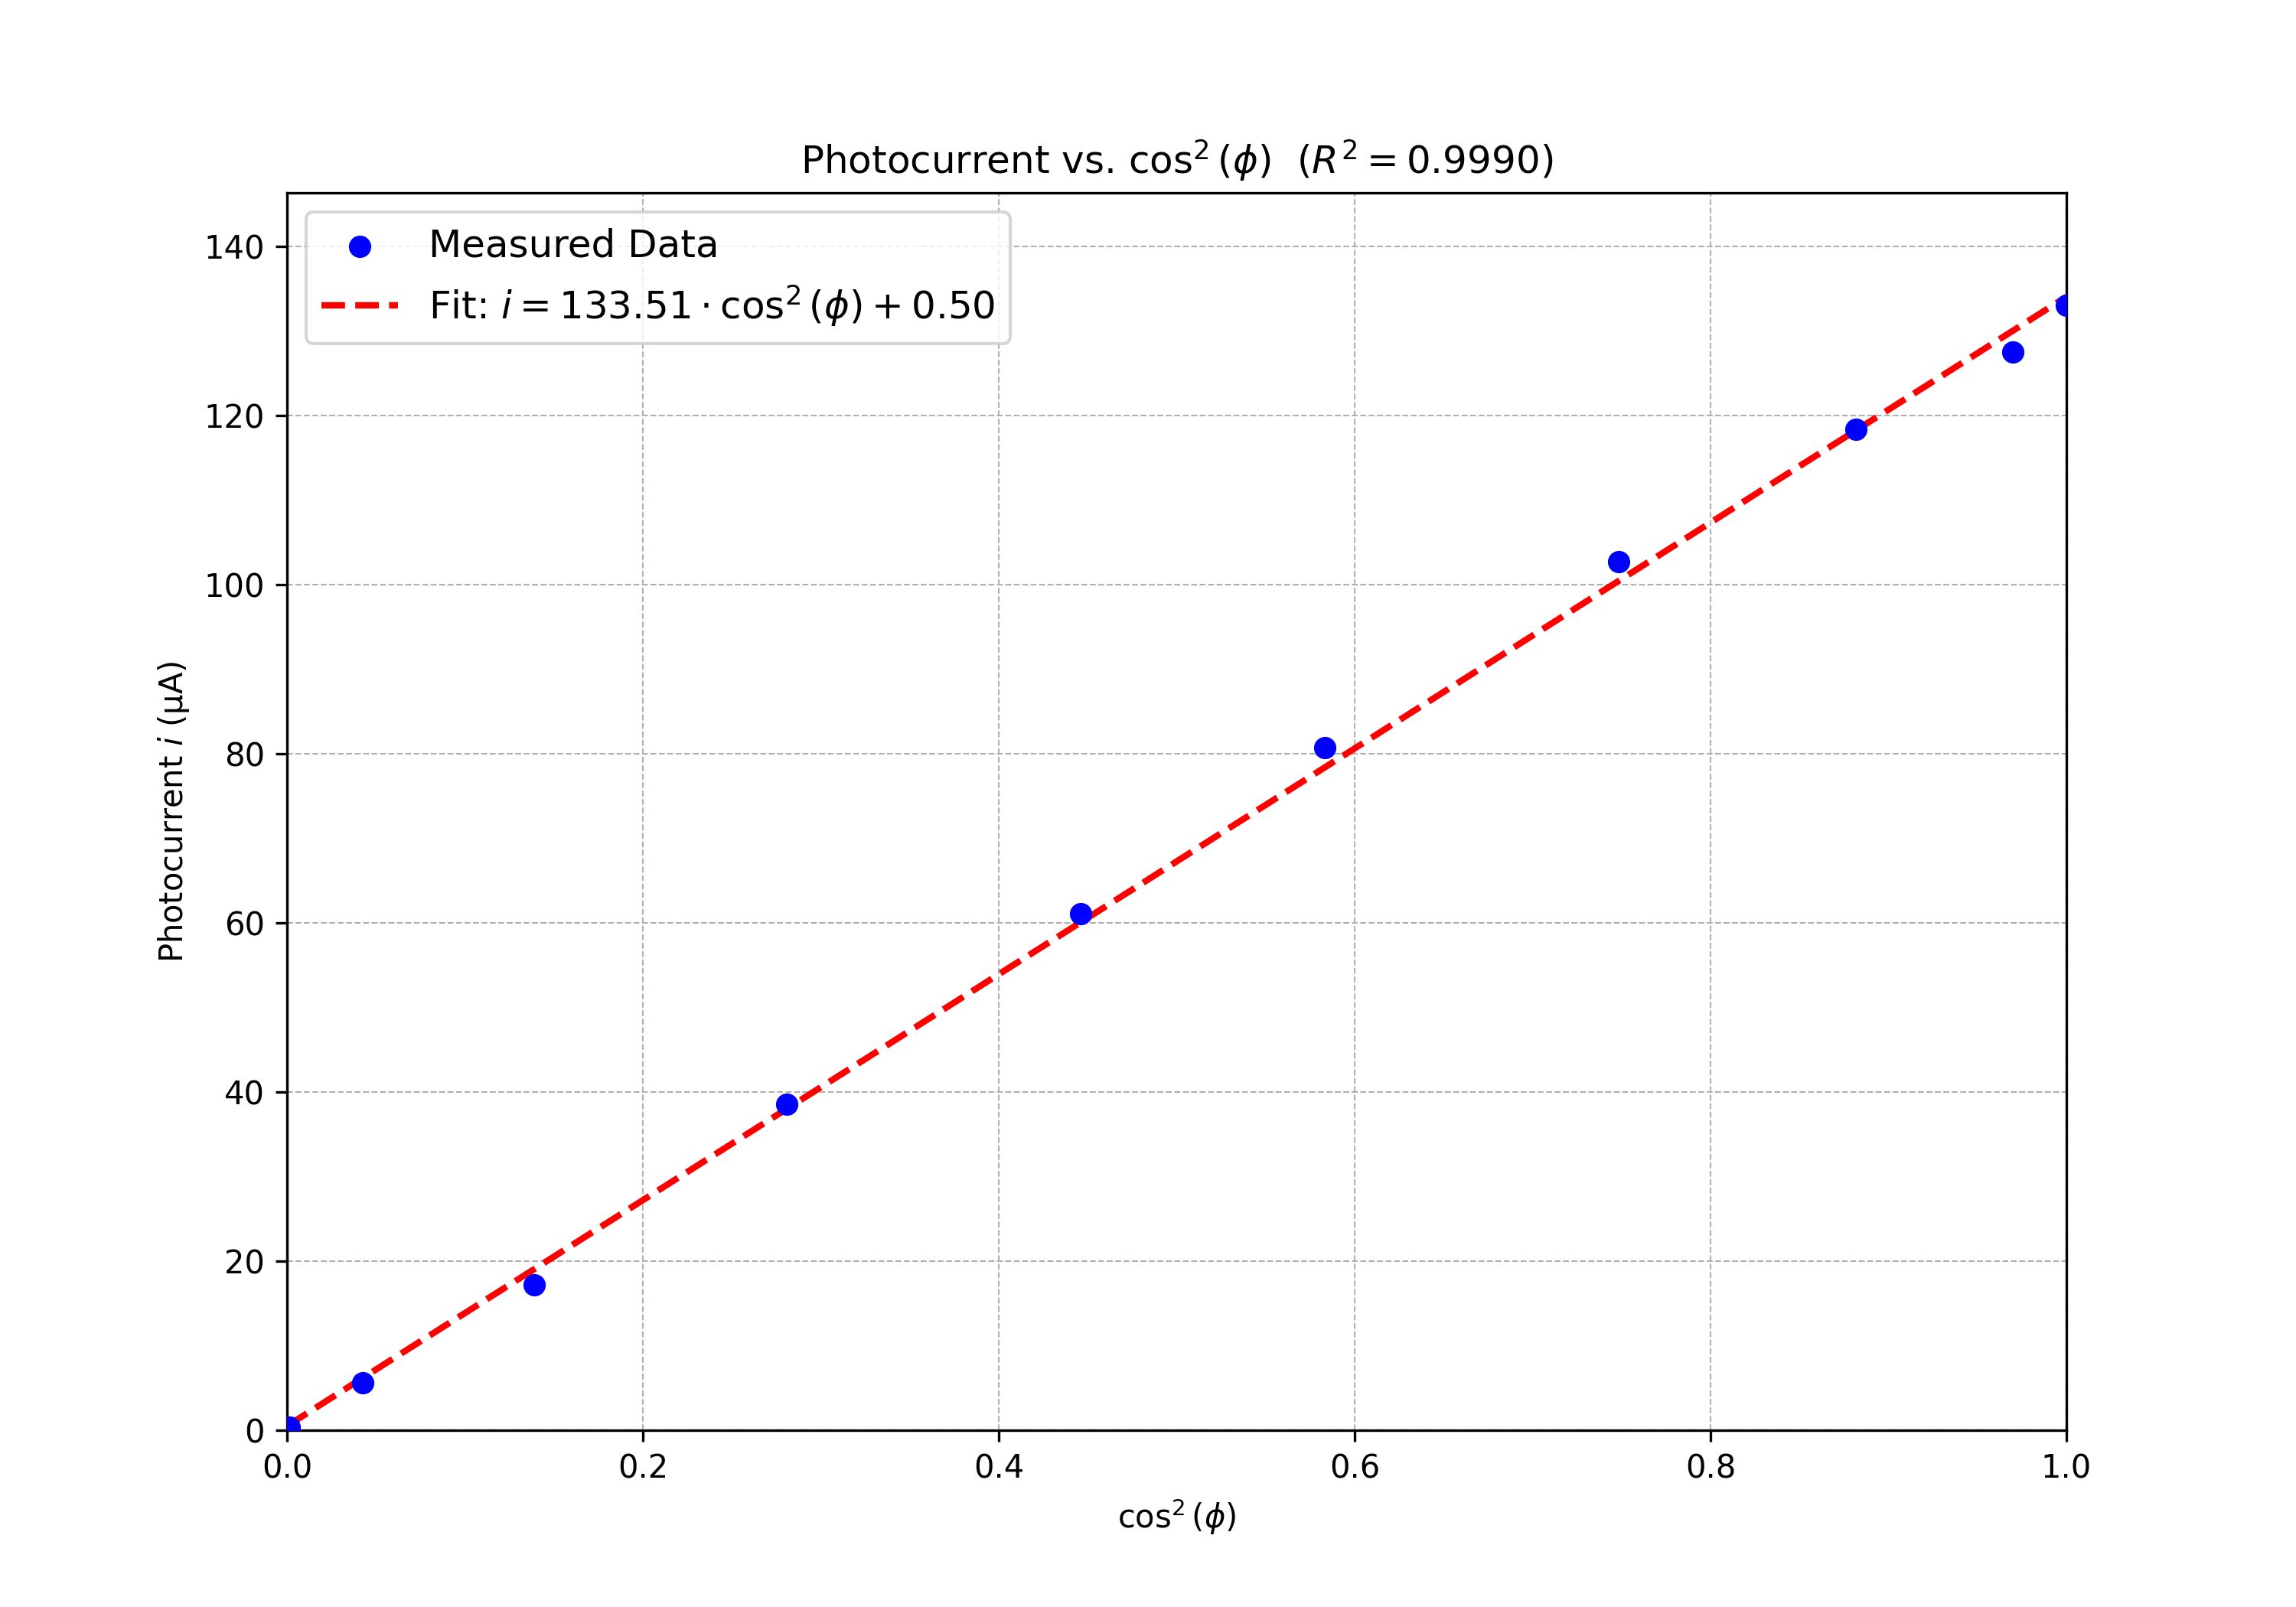
\includegraphics[width=0.7\textwidth]{figure/i_pi.png}
    \caption{光电流与${\cos ^2 \phi}$的关系曲线}
\end{figure}
拟合方程为：
\[
i = 133.51{\cos ^2 \phi}+0.50
\]
$R^2=0.9990$大于0.99，说明拟合效果很好，表明硅光电池可以将偏振光的光强线性地转化为光电流大小。
    \myspace{2}
\section{误差分析}
\xiaosi（运用测量误差、相对误差、不确定度等分析实验结果，20分）

\subsection{测量黑色平板折射率的误差分析}

\subsubsection{系统误差}
\begin{enumerate}
    \item \textbf{仪器误差}：分光仪的最小分度为\SI{0.1}{\degree}，其B类不确定度为\SI{0.0577}{\degree}
    \item \textbf{对中误差}：望远镜与平行光管未能完全对中，导致角度读数偏差
    \item \textbf{视差误差}：人眼读数时存在视差，特别是在判断光强最小时存在主观判断误差
    \item \textbf{平台水平误差}：分光仪平台未能完全水平，影响角度测量的准确性
\end{enumerate}

\subsubsection{随机误差}
\begin{enumerate}
    \item \textbf{测量重复性}：6次测量的布儒斯特角标准偏差为\SI{0.3113}{\degree}
    \item \textbf{环境因素}：环境光变化、空气扰动等影响光强判断
    \item \textbf{操作稳定性}：手动转动望远镜时存在的微小抖动
\end{enumerate}

\subsubsection{折射率不确定度分析}
最终折射率测量结果为：
\[
n = 1.375 \pm 0.007
\]
相对不确定度：
\[
\frac{u_n}{n} = \frac{0.007}{1.375} = 0.51\%
\]

\subsection{偏振片偏振化角度测量的误差分析}

\subsubsection{数据异常分析}
实验中第3个测量值\ang{79.5}明显异常，可能原因：
\begin{enumerate}
    \item \textbf{读数错误}：可能误读了刻度盘
    \item \textbf{偏振片滑动}：在转动过程中偏振片位置发生变化
    \item \textbf{环境干扰}：测量时受到外部光干扰
    \item \textbf{判断失误}：在寻找极值时判断错误
\end{enumerate}

\subsubsection{有效数据处理结果}
舍去异常值后，7个有效测量值的标准差为\SI{0.97}{\degree}，表明数据一致性较好。最终结果为：
\[
\theta = (72.4 \pm 0.4)^\circ
\]
相对不确定度：
\[
\frac{u_\theta}{\bar{\theta}} = \frac{0.4}{72.4} = 0.55\%
\]

\subsection{探究光电流与光强关系的误差分析}

\subsubsection{拟合质量分析}
光电流与$\cos^2\phi$的线性拟合决定系数$R^2=0.9990$，表明：
\begin{enumerate}
    \item \textbf{线性关系良好}：光电流与光强呈高度线性关系
    \item \textbf{测量精度高}：数据点基本落在拟合直线上
    \item \textbf{实验成功}：验证了硅光电池能将光强线性地转化为光电流
\end{enumerate}

\subsubsection{残差分析}
\begin{enumerate}
    \item \textbf{系统偏差}：截距项\SI{0.50}{\micro\ampere}可能源于暗电流或背景光
    \item \textbf{非线性因素}：在光强较弱时，硅光电池可能存在轻微非线性响应
\end{enumerate}

\section{实验探讨}
\xiaosi（对实验内容、现象和过程的小结，不超过100字，10分）

本实验通过布儒斯特角法成功测量了黑色平板的折射率$n=1.375\pm0.007$，测量精度较高。
在偏振片偏振化方向测量中，发现并正确处理了一个异常数据点，最终得到可靠结果$(72.4\pm0.4)^\circ$。
通过验证马吕斯定律，证实了硅光电池的光电流与入射光强呈良好线性关系（$R^2=0.9990$），实验装置和测量方法合理有效。
实验中的主要误差来源为角度读数的随机误差和仪器本身的系统误差。

\section{思考题}
\xiaosi（解答教材或讲义或老师布置的思考题，10分）

1.请简述减小实验误差的方法？

\textbf{（1）减小系统误差：}
\begin{itemize}
    \item 使用更高精度的测量仪器（如电子角度计代替机械分光仪）
    \item 定期校准仪器，确保零点准确
    \item 改进实验装置，减少光路中的杂散光
    \item 使用激光光源代替普通光源，提高光束方向性
\end{itemize}

\textbf{（2）减小随机误差：}
\begin{itemize}
    \item 增加测量次数，采用多次测量取平均值
    \item 改善实验环境，减少震动和空气扰动
    \item 采用数据记录自动化，减少人为读数误差
    \item 在稳定条件下进行测量，避免外界干扰
\end{itemize}

\textbf{（3）提高操作技巧：}
\begin{itemize}
    \item 熟练实验操作，减少人为操作误差
    \item 采用对称测量法消除系统误差
    \item 多人重复测量，交叉验证结果
\end{itemize}
\myspace{2}
2.在探究光电流与光照强度关系时背景光照的影响是怎样的？

\textbf{背景光照的影响及应对措施：}
\begin{enumerate}
    \item \textbf{产生暗电流}：背景光会使硅光电池产生额外的暗电流，影响弱光信号的测量
    \quad \textbf{对策}：实验前测量并扣除暗电流值，或在暗室中进行实验
    
    \item \textbf{降低信噪比}：背景光噪声会掩盖微弱的光信号变化
    \quad \textbf{对策}：使用遮光罩、暗箱等屏蔽环境光
    
    \item \textbf{造成测量偏差}：特别是在验证马吕斯定律时，背景光会导致光电流与$\cos^2\phi$关系的截距不为零
    \quad \textbf{对策}：拟合时考虑非零截距，或测量前先扣除背景光影响
    
    \item \textbf{影响线性范围}：强背景光可能使硅光电池接近饱和，破坏线性响应
    \quad \textbf{对策}：控制背景光强度，确保工作在线性区
\end{enumerate}
\myspace{2}
3.下列哪些波能发生偏振现象(B)

\begin{itemize}
    \item \textbf{A. 声波} ❌ 声波是纵波，振动方向与传播方向平行，不会发生偏振现象
    \item \textbf{B. 电磁波} ✅ 电磁波是横波，电场和磁场振动方向垂直于传播方向，可以发生偏振现象
    \item \textbf{C. 地震波P波} ❌ P波是纵波，不会发生偏振现象
    \item \textbf{D. 水波} ❌ 水波既不是纯粹的纵波也不是纯粹的横波，但一般不能发生明显的偏振现象
\end{itemize}
\myspace{2}

4.如何调整两块平行放置的偏振片的透振方向，让通过的太阳光透射光强度获得最大值和最小值？

\textbf{（1）获得最大透射光强：}
将两块偏振片的透振方向调整到相互平行。设入射的自然光强度为$I_0$，则通过第一块偏振片后的线偏振光强度为$I_1 = \frac{1}{2}I_0$（马吕斯定律，自然光通过偏振片强度减半）。当第二块偏振片透振方向与第一块平行时，透射光强$I_2 = I_1 = \frac{1}{2}I_0$，为最大值。

\textbf{（2）获得最小透射光强（消光）：}
将两块偏振片的透振方向调整到相互垂直（夹角\ang{90}）。此时，通过第一块偏振片的线偏振光无法通过第二块偏振片，透射光强$I_2 = I_1\cos^2(90^\circ) = 0$，实现完全消光。

\textbf{实际操作步骤：}
\begin{enumerate}
    \item 固定第一块偏振片
    \item 旋转第二块偏振片，观察透射光强变化
    \item 当透射光最强时，两块偏振片透振方向平行
    \item 继续旋转\ang{90}，当透射光最弱（基本看不到光）时，两块偏振片透振方向垂直
\end{enumerate}
\newpage

\sihao\textbf{注意事项：}
\xiaosi
\begin{enumerate}
    \item 用PDF格式上传“实验报告”，文件名：学生姓名+学号+实验名称+周次。
    \item  “实验报告”必须递交在“学在浙大”的本课程的对应实验项目的“作业”模块内。
    \item  “实验报告”成绩必须在“浙江大学物理实验教学中心网站”-“选课系统”内查询。
    \item 教学评价必须在“浙江大学物理实验教学中心网站”-“选课系统”内进行，学生必须进行教学评价，才能看到实验报告成绩，教学评价必须在本次实验结束后 3 天内进行。
\end{enumerate}

\vspace{1cm}
\xiaosi\centering \textbf{浙江大学物理实验教学中心制}

\end{document}